\section{Hardware components}
\label{sec:hardwareComponents}
In the very beginning of the project, the team looked into the possibility of getting live data directly from devices. This required some technical equipment for collecting and transmitting power usage from a device. This section describes the architecture and the necessary hardware.

\subsection{Hardware architecture}

The envisioned architecture is shown in figure~\ref{fig:idealArchitecture}. This includes both finished functionality and the concepts the team were unable to implement because of technical restrictions or time constraints. The team concluded that the best architecture for a such a system would include a home data aggregator. The home data aggregator recieves data from the measuring units connected with the devices. Depending on the functionality of the measuring units, remotely controlling devices, can be possible.

\begin{figure}[H]
\centering
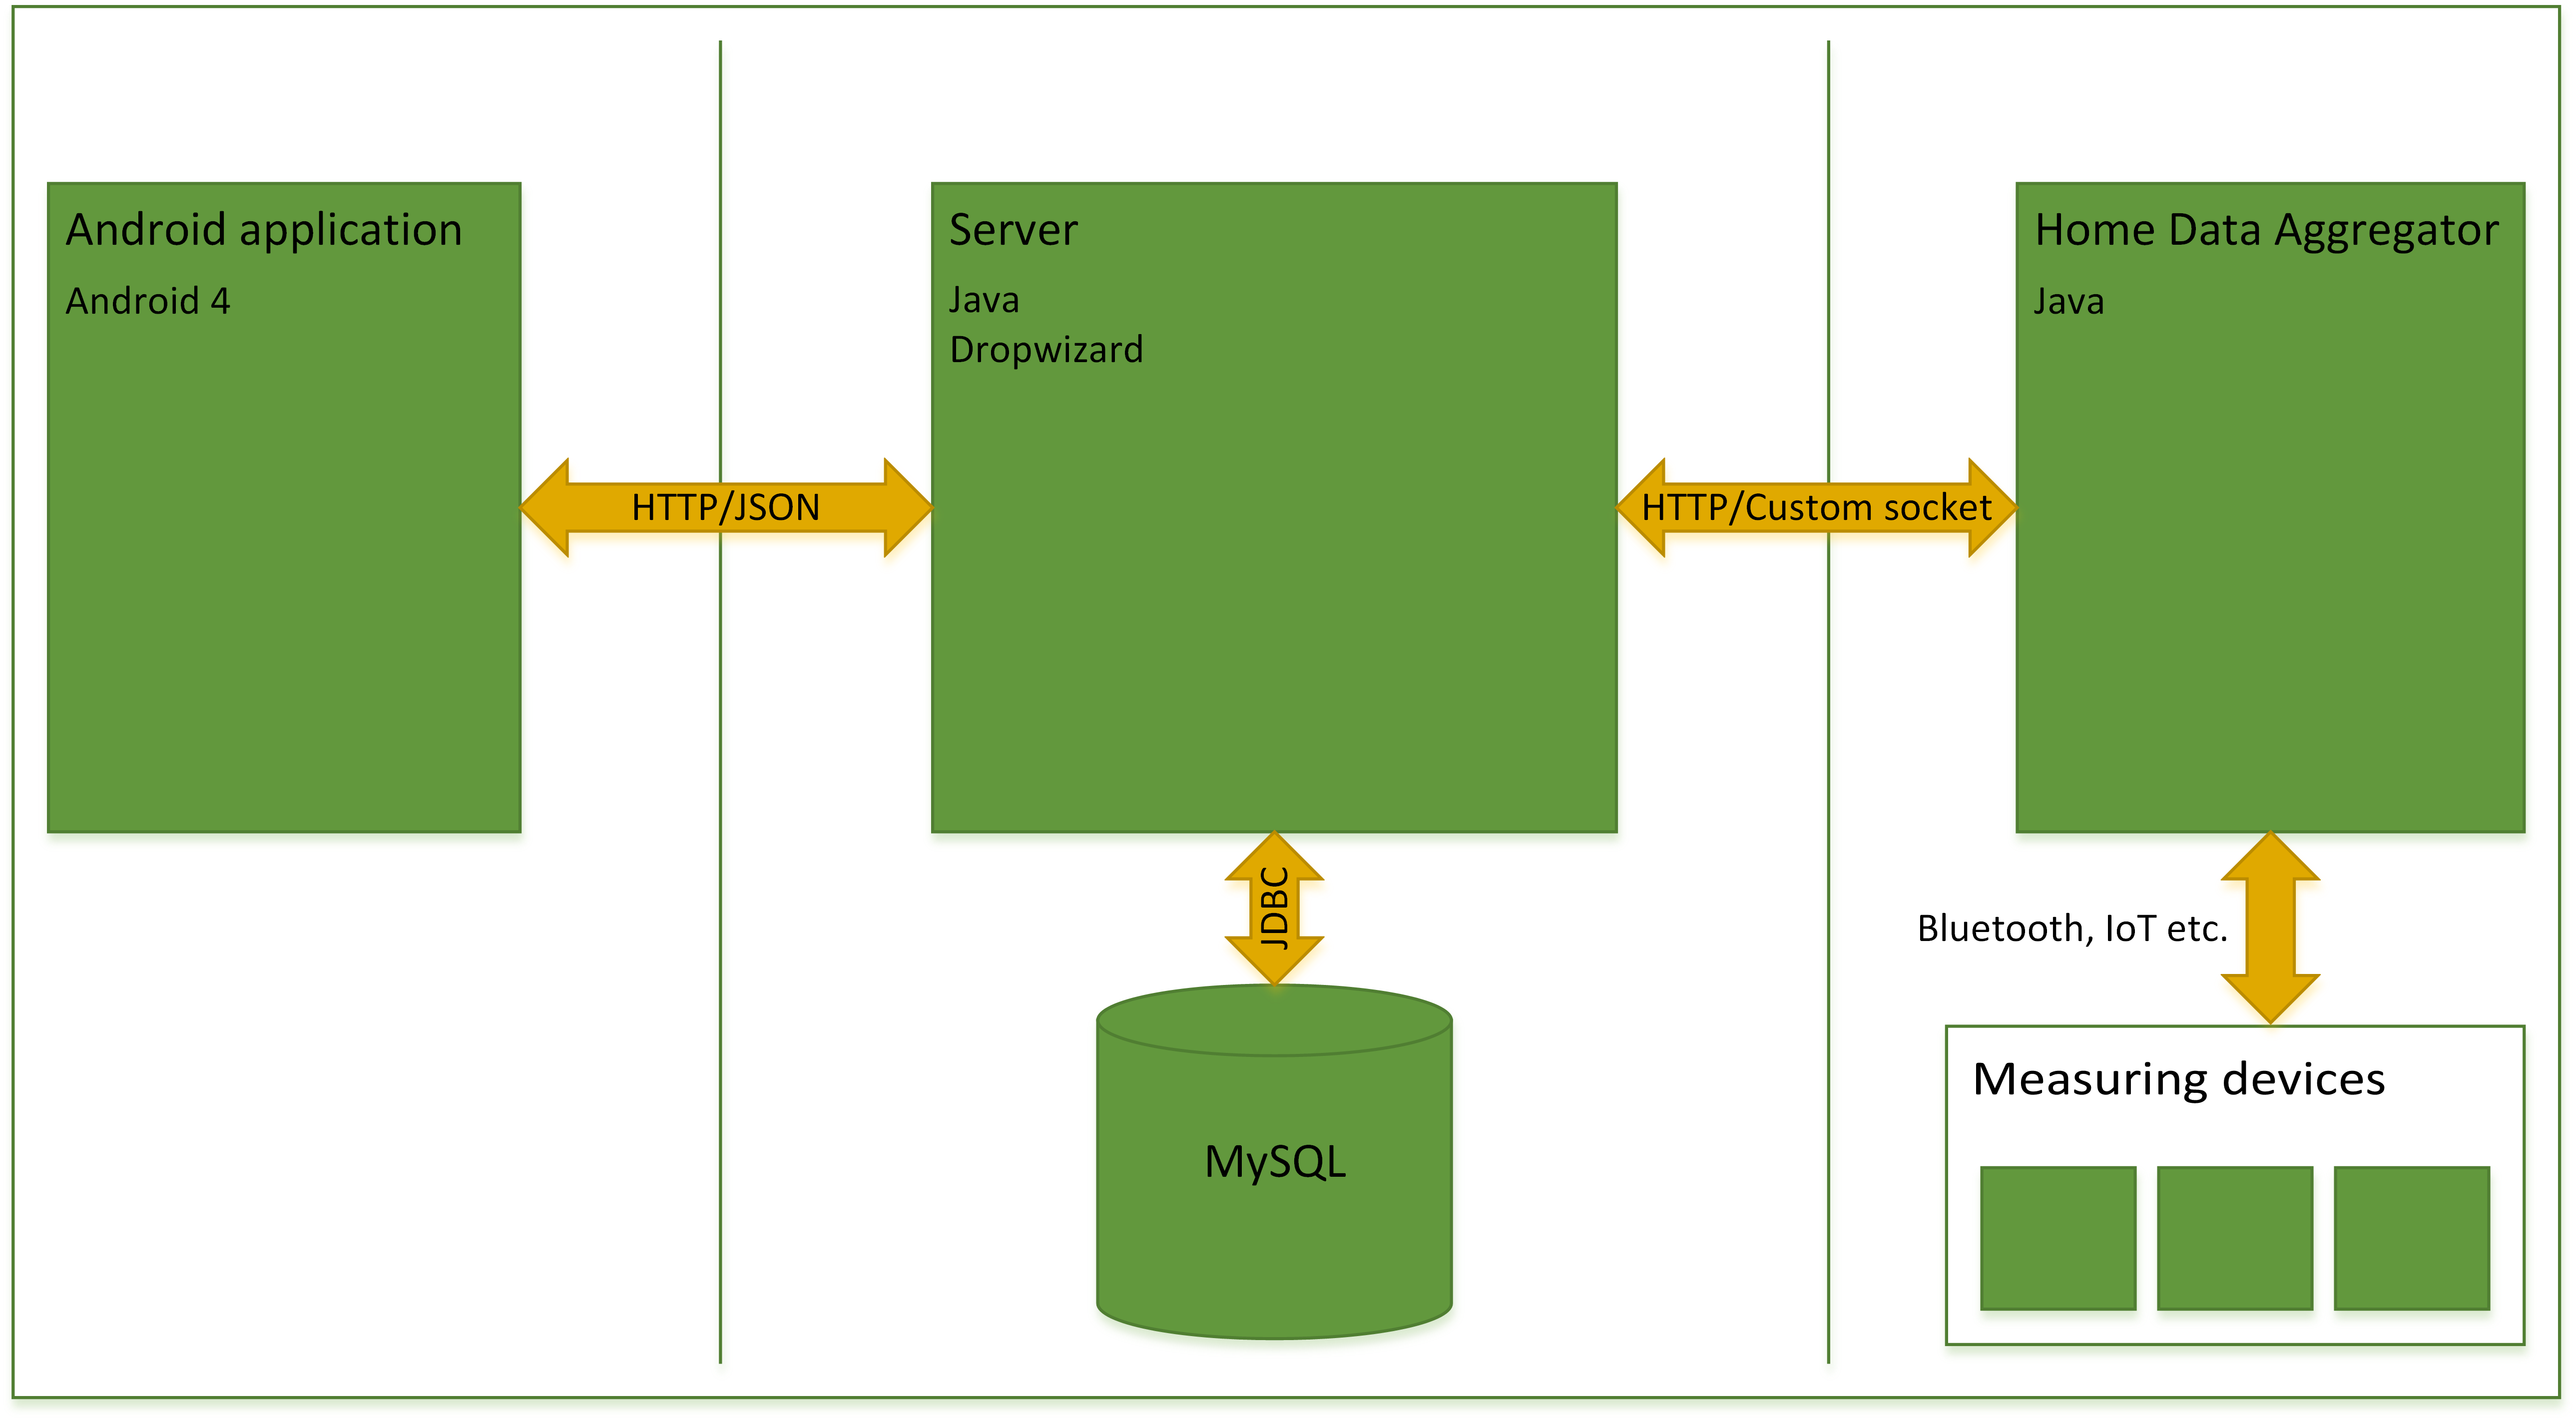
\includegraphics[width=\textwidth]{ch/further/fig/architecture.png}
\caption{Ideal Wattitude architecture}
\label{fig:idealArchitecture}
\end{figure}


\subsection{Home data aggregator}
To ensure full operability 24 hours a day, a base station is needed in the user's home. This server will serve as an aggregating agent for data from measuring units attached to devices. Given an ideal architecture implementation, this unit would also be responsible for controlling devices. The team envisions this unit as a synchronization service working for the Wattitude cloud server. The software for such a server could be based on the current server software. The hardware for this base station could be as simple as a Raspberry Pi~\cite{pi}. These computers are small, cheap and provides all the hardware needed for a simple home aggregator. Some modifications is necessary to communicate with the measuring units. The architecture for this aggregation unit is shown in figure~\ref{fig:aggregator}.

\begin{figure}[H]
\centering
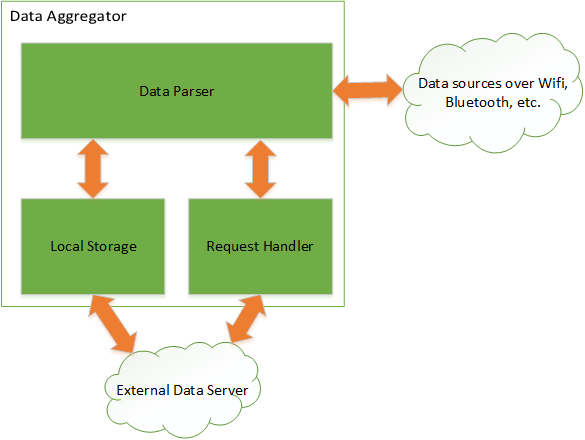
\includegraphics[width=\textwidth]{ch/further/fig/home.png}
\caption{Detailed architecture for the home data aggregator}
\label{fig:aggregator}
\end{figure}

\subsection{Measuring unit}
To make real time monitoring possible, every device the user wants to monitor must be connected to a wireless monitoring unit. The team tried to find an existing solution that was satisfying, but most of the options found was proprietary and/or too expensive. The following paragraphs describes the most viable options.

\subsubsection{HomeMatic plug}
This is the device that the CoSSMic team at SINTEF has been experimenting with. The drawbacks is that it has a unit price of almost 500 NOK and must be imported. Covering most home devices with such a measuring device would be extremely costly. As hardware devices were not a part of the project scope, the team did not do any research on how to interface with this unit. More detailes about this can be found in Appendix~ref{sec:homematic}.

\subsubsection{Do It Yourself (DIY) Arduino}
A much cheaper, but perhaps limited solution, is one from Open Energy Monitor~\cite{oemmodule}. These units do not support the ability to control devices, only measurement of consumption. They are much cheaper than the HomeMatic unit, but must be assembled manually. The unit can be good for experimenting and prototyping but it is far from ready for the home market.


